\documentclass[oneside,final,14pt]{extreport}
\usepackage[utf8]{inputenc}
\usepackage[russianb]{babel}
\usepackage{vmargin}
\setpapersize{A4}
\setmarginsrb{3cm}{2cm}{1cm}{2cm}{0pt}{0mm}{0pt}{13mm}
\usepackage{indentfirst}
\usepackage{graphicx}
\sloppy



\begin{document}
	
	
	
	%\setcounter{secnumdepth}{-1} % чтоб не нумеровались главы
	
	Аннотация: Аннотация работы может содержать не более 1500 знаков. Пишется отдельно.
	
	\tableofcontents
	
	\chapter*{Введение}
	
	\section{Про принтинг}
	




\section{Про СЛС И материалы для него}
The main advantages of SLS over other technologies of additive production are the following: 1) products produced by the SLS method are similar in properties of polymeric materials obtained using standard methods such as extrusion, injection molding, hot pressing, etc.; 2) theoretically, any material that can be transferred in a powder state and melted at increasing temperature can be processed using SLS technology; 2 3) the absence of any additional supporting element when printing complex products.

The properties of the final product obtained by the SLS technology largely depend on the properties of the original powder (morphology, size, size distribution, bulk density, thermal properties, viscosity and surface tension) and on the parameters of laser sintering (laser power, scanning speed, laser spot diameter). Particle morphology affects the spatial arrangement of powder particles (stacking degree) relative to each other. Spherical (with a smooth surface) particles have a high packing density. They provide flowability of the powder composition in systems of applying the material with minimal resistance. In addition, spherical particles are well bonded in the process of laser sintering. It was shown that during the transition from powder particles with predominantly spherical morphology to particles of irregular shape of the same material, the elastic modulus decreases by almost 40 \%.3 The spherical particles with good flowability and a high packing densities represent ideal characteristics of the starting powder for use in SLS.4 At the same time, the use of irregularly shaped particles with a large variation in their size leads to the creation of products with higher mechanical characteristics, compared to the use of mainly spherical particles with a narrow size distribution.5
	
	Researches on the application of other polymers in SLS technology are very limited. In addition to polyamide, polystyrene and polycarbonate are used as a starting material for SLS.12,13
	[vaganov corrected]
	
	\section{Про ПИ}
	
	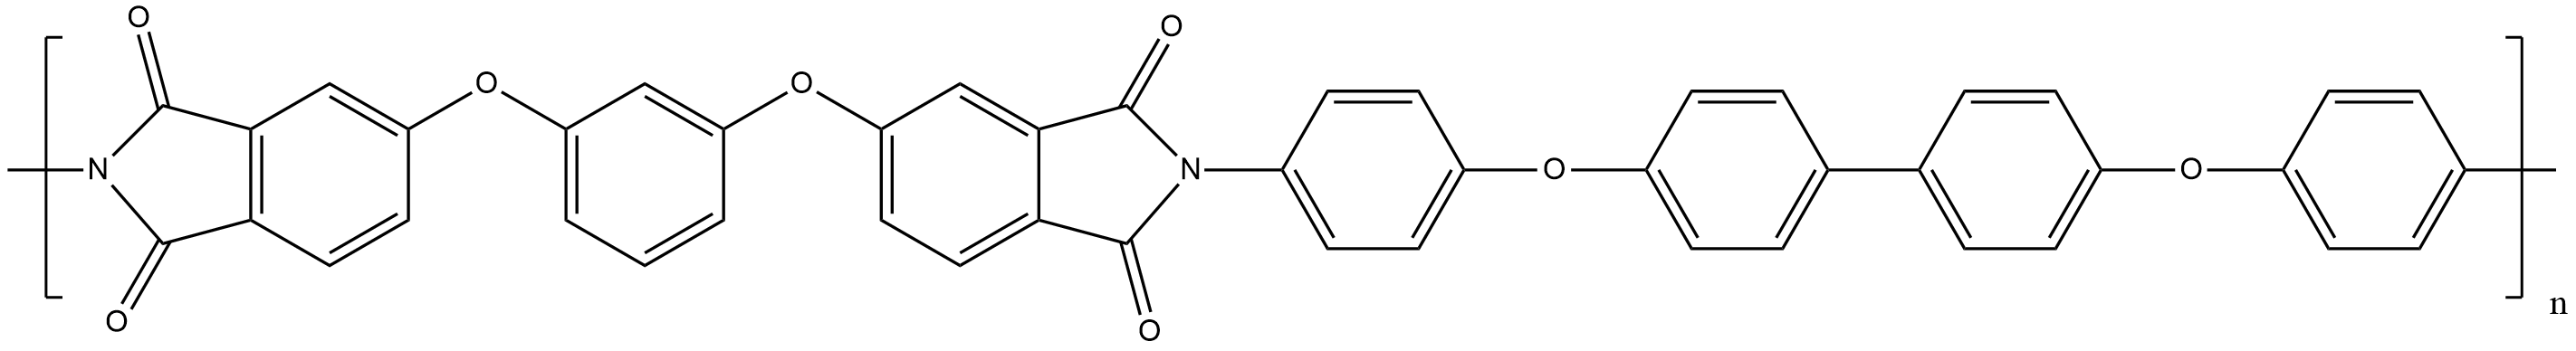
\includegraphics[width=\textwidth]{formula.png}
	
	ПИ это круто и вот почему:
	Свойства: глава1
	Полиимиды: глава10
	[Михайлин. Термоустойчивые полимеры и полимерные материалы]
	
	
	
	***
	
	
	"Анализ современной литературы показывает, что на сегодняшний день исследования в области приме-нения термостойких полимеров для СЛС сосредоточе-ны лишь на семействе полиэфиркетонов [Berretta S., Ghita O., Evans K. E. // European Polymer Journal, 2014. Vol. 59. P. 218–229]. На данный момент практически отсутствуют сведения об использовании других клас-сов термостойких полимеров, таких, например, как полиимиды (ПИ). Кроме того, существует ряд проти-воречивых сведений о влиянии тех или иных параметров на процесс СЛС и конечные свойства материала в целом. В связи с этим, с научной и технической точки зрения весьма перспективным представляется иссле-дование закономерностей формирования структуры при СЛС порошков ПИ, изучение процесса их сплав-ления в зависимости от свойств порошка, содержания нанонаполнителей, а также параметров СЛС.
	В ИВС РАН синтезированы термопластичные частично кристаллические ПИ гомологического ряда Р-ОДФО на основе отечественного резорцинового диангидрида Р (1,3-бис-(3,3,4,4-дикарбоксифенокси)-бензол) и четырехядерного диамина ОДФО (4,4-бис(4-аминофенокси)бифенил) методом химической (с использованием катализаторов) и термической имидизации [Юдин В. Е., Светличный В. М. // Высоко-молекулярные соединения, серия С, 2016. Т. 58. №1. С. 19]. Исследованы форма, размер частиц (фракци-онный состав ПИ порошка). Показано, что методом химической имидизации формируются порошки с более узким распределением частиц по размерам (6–10 мкм), по сравнению с термически имидизованным порошком, а при увеличении молекулярной массы и дополнительной термообработки возрастает их насыпная плотность (до 0,5 г/мл), что способствует улучшению механических характеристик изделий, формируемых по методу СЛС. Важно отметить, что с увеличением молекулярной массы ПИ наблюдается резкое возрастание вязкости его расплава, что препят-ствует слиянию частиц в процессе СЛС.
На основе ПИ порошка Р-ОДФО впервые мето-дом СЛС получены образцы в виде пленок. Исследо-ваны свойства образцов в зависимости от способа синтеза, молекулярной массы и мощности лазера и показано, что более однородная и плотная структу-ра плёнок с относительно высокими механическими характеристиками получается из порошков, синтези-руемых по методу химической имидизации.
	"[ПОЛИМЕРНЫЕ МАТЕРИАЛЫ И ТЕХНОЛОГИИ Т.4 (2018), №3, 5
Редакционная колонка — личное мнение
Полиимидные порошки для 3D-печати по методу СЛС]
	
	
	***
	
	"Therefore the promising direction in SLS is using of high-performance thermostable
thermoplastic polymers and polymer’s modification with small additives of nanoparticles.
The specially designed laser sintering system was used for processing single layer film from powder particles by SLS. Obtained
samples were characterized by using mechanical testing machine.
The mechanical properties of all the samples were studied depending on power of the laser; the values of tensile strength, modulus of
elasticity and deformation at break were determined. The effect of carbon nanoparticles introduction in polyimide on the size, shape,
fractional composition of the powder andthe mechanical properties of the sintered samples will be discussed"
[SYNTHESIS AND INVESTIGATION OF NANOMODIFED POLYIMIDE POWDER FOR
SELECTIVE LASER SINTERING
Vaganov G.V.1, Didenko A.L.1, Polyakov I.V.2, Ivan’kova E.M.1, Popova E.N.1, Yudin V.E.1,2 MODERN PROBLEMS
OF POLYMER SCIENCE
Program and Abstract Book
of 14th International Saint Petersburg Conference
of Young Scientists]	

\section{А при чем тут структура?}
+цели и задачи


	\addcontentsline{toc}{chapter}{Введение}
	
	\chapter*{Список обозначений и сокращений}
	
	СИ -- синхротронное излучение\\
	Р-ОДФО -- наш полимер\\
	WAXS -- широкоугловое рассеяние\\
	и тд и тп
	
	\chapter{Теория}
	
	
	
	\chapter{Эксперимент}
	
	\section{Материалы}
	
	Свойства и результаты прочих исследований:
	[Vaganov corrected]
	
	
	
	\chapter*{Заключение}
	\addcontentsline{toc}{chapter}{Заключение}
	
	
	%bibliography
	\addcontentsline{toc}{chapter}{Литература}
	
\end{document}